\chapter{考察}
\label{cha:Discussion}

本研究では、既存ツールの有用性の向上を目的として、自然言語仕様書からクラス、操作定義、操作定義を生成する手法を提案し、
既存ツールに適用することによってVGMLを開発した。
本章では、VGMLに関して考察する。

\section{VGMLの有用性}
本節では、VGMLが自然言語仕様書から生成したVDM++仕様書を、正解のVDM++仕様書と比較して評価する。ここで、正解のVDM++仕様書として、
著者が仕様書Aと仕様書Bから人手によって記述したVDM++仕様書を用いる。
仕様書Aから人手によって記述したVDM++仕様書は、6つのファイルで構成し、仕様書Bから人手によって記述したVDM++仕様書は、7つのファイルで構成する。
仕様書Aから作成したVDM++仕様書を、図\ref{fig:speA_vdm1}-図\ref{fig:speA_vdm6}に、仕様書Bから作成したVDM++仕様書を、図\ref{fig:speB_vdm1}-図\ref{fig:speB_vdm7}に示す。

正解のVDM++仕様書は、以下の条件に基づいて作成した。

\begin{itemize}
    \item 自然言語仕様書内で属性や振る舞いを持ち、自然言語仕様書が対象とするシステムの外部に位置するアクターではない名詞を、クラスとして定義する。
    \item システム内で数字などの不変の情報を持つ名詞を定数名とし、当該名詞が持つ情報を値として定義する。
    \item あるクラスの候補となる名詞が持つ情報であり、クラスが振る舞いを行う際に必要とする情報である名詞を、当該クラスの候補である名詞の持つインスタンス変数として定義する。
    \item あるクラスの候補となる名詞が行う振る舞いを表す名詞であり、かつ、インスタンス変数定義の候補である名詞を参照する名詞。
\end{itemize}

今回は、VGMLの有用性の評価のために、VGMLが生成したVDM++仕様書内の単語と、正解のVDM++仕様書内の単語についてのF値を測定した。
F値は、適合率と再現率の調和平均である。F値の計算式を、以下に示す。

\begin{equation}
    \mbox F値=\frac{2 \times 適合率 \times 再現率}{適合率+再現率}
\end{equation}	

評価する項目を、以下に示す。

\begin{itemize}
    \item クラスに対する評価
    \item インスタンス変数定義に対する評価
    \item 操作定義に対する評価
\end{itemize}

以降、それぞれの評価について示す。

\subsection{クラスに対する評価}
VGMLが生成するVDM++仕様書におけるクラスと、正解のVDM++仕様書におけるクラスを比較し、一致したクラスをF値を用いて評価する。
クラスに対する評価の適合率は、VGMLが生成したクラスのうち、正解のVDM++仕様書のクラスと一致したクラスの数との割合であり、
再現率は正解のVDM++仕様書のクラスのうち、VGMLが生成したクラスと一致したクラスの数との割合である。
以下に、クラスに対する評価の適合率、再現率の計算式を、それぞれ示す。

\begin{equation}
    \mbox 適合率=\frac{正解の\mathrm{VDM\!+\!+}仕様書のクラスと一致したクラスの数}{VGMLが出力したクラスの数}
\end{equation}
\begin{equation}
    \mbox 再現率=\frac{正解の\mathrm{VDM\!+\!+}仕様書のクラスと一致したクラスの数}{正解の\mathrm{VDM\!+\!+}仕様書のクラスの数}
\end{equation}

VGMLが生成したVDM++仕様書におけるクラスと、正解のVDM++仕様書におけるクラスを比較した際の実験結果を、表\ref{table:classResult}に示す。

表\ref{table:classResult}より、VGMLは、抽出した単語をクラスとして出力する際に、仕様書AでF値1.0、仕様書BでF値0.72の精度で出力できた。
このことにより、VGMLは、教師データの自然言語仕様書と異なる自然言語仕様書に対しても、一定の割合でVDM++仕様書におけるクラスを生成できることがわかる。
よって、VGMLは、既存ツールの有用性を向上できたといえる。


\begin{table}[t]
	\caption{VGMLが生成したVDM++仕様書におけるクラスと正解のVDM++仕様書におけるクラスを比較した際の実験結果}
	\label{table:classResult}
	\begin{center}
        \begin{tabular}{c|c|c|c|c|c|c}
            \hline
            仕様書  & 正解の & 出力した & 一致した & 適合率 & 再現率 & F値  \\
                    & VDM++仕様書 & VDM++仕様書 &         &        &       &      \\
                    & のクラスの数 & のクラスの数 & クラスの数  &        &       &      \\
            \hline
            仕様書A & 5                             & 5                 & 5                  & 1.0   & 1.0    & 1.0  \\
            \hline
            仕様書B & 6                             & 5                  & 4                  & 0.8   & 0.67   & 0.72 \\
            \hline
        \end{tabular}
    \end{center}
\end{table}

\subsection{インスタンス変数定義に対する評価}
VGMLが生成するVDM++仕様書におけるインスタンス変数定義と、正解のVDM++仕様書におけるインスタンス変数定義を比較し、一致したインスタンス変数定義をF値を用いて評価する。
インスタンス変数定義に対する評価の適合率は、VGMLが生成したインスタンス変数定義のうち、正解のVDM++仕様書のインスタンス変数定義と一致したインスタンス変数定義の数との割合であり、
再現率は正解のVDM++仕様書のインスタンス変数定義のうち、VGMLが生成したインスタンス変数定義と一致したインスタンス変数定義の数との割合である。
以下に、インスタンス変数定義に対する評価の適合率、再現率の計算式を、それぞれ示す。

\begin{equation}
    \mbox 適合率=\frac{正解の\mathrm{VDM\!+\!+}仕様書のインスタンス変数定義と一致したインスタンス変数定義の数}{VGMLが出力したインスタンス変数定義の数}
\end{equation}
\begin{equation}
    \mbox 再現率=\frac{正解の\mathrm{VDM\!+\!+}仕様書のインスタンス変数定義と一致したインスタンス変数定義の数}{正解の\mathrm{VDM\!+\!+}仕様書のインスタンス変数定義の数}
\end{equation}

VGMLが生成したVDM++仕様書におけるインスタンス変数定義と、正解のVDM++仕様書におけるインスタンス変数定義を比較した際の実験結果を、表\ref{table:instanceResult}に示す。

表\ref{table:instanceResult}より、VGMLは、抽出した単語をインスタンス変数定義として出力する際に、仕様書AでF値0.62、仕様書BでF値0.61の精度で出力できた。
このことにより、VGMLは、教師データの自然言語仕様書と異なる自然言語仕様書に対しても、一定の割合でVDM++仕様書におけるインスタンス変数定義を生成できることがわかる。
よって、VGMLは、既存ツールの有用性を向上できたといえる。

\begin{table}[t]
	\caption{VGMLが生成したVDM++仕様書におけるインスタンス変数定義と正解のVDM++仕様書におけるインスタンス変数定義を比較した際の実験結果}
	\label{table:instanceResult}
	\begin{center}
        \begin{tabular}{c|c|c|c|c|c|c}
            \hline
            仕様書  & 正解の & 出力した &  & 適合率 & 再現率 & F値  \\
                    & VDM++仕様書の & VDM++仕様書の & 一致した  &        &       &      \\
                    & インスタンス & インスタンス & インスタンス  &        &       &      \\
                    & 変数定義の数 & 変数定義の数 & 変数定義の数  &        &       &      \\
            \hline
            仕様書A & 20                             & 9                 & 9                  & 1.0   & 0.45    & 0.62  \\
            \hline
            仕様書B & 26                             & 20                  & 14                  & 0.7   & 0.54   & 0.61 \\
            \hline
        \end{tabular}
    \end{center}
\end{table}

\subsection{操作定義に対する評価}
VGMLが生成するVDM++仕様書における操作定義と、正解のVDM++仕様書における操作定義を比較し、一致した操作定義をF値を用いて評価する。
操作定義に対する評価の適合率は、VGMLが生成した操作定義のうち、正解のVDM++仕様書の操作定義と一致した操作定義の数との割合であり、
再現率は正解のVDM++仕様書の操作定義のうち、VGMLが生成した操作定義と一致した操作定義の数との割合である。
以下に、操作定義に対する評価の適合率、再現率の計算式を、それぞれ示す。

\begin{equation}
    \mbox 適合率=\frac{正解の\mathrm{VDM\!+\!+}仕様書の操作定義と一致した操作定義の数}{VGMLが出力した操作定義の数}
\end{equation}
\begin{equation}
    \mbox 再現率=\frac{正解の\mathrm{VDM\!+\!+}仕様書の操作定義と一致した操作定義の数}{正解の\mathrm{VDM\!+\!+}仕様書の操作定義の数}
\end{equation}

VGMLが生成したVDM++仕様書における操作定義と、正解のVDM++仕様書における操作定義を比較した際の実験結果を、表\ref{table:operateResult}に示す。

表\ref{table:operateResult}より、VGMLは、抽出した単語を操作定義として出力する際に、仕様書AでF値0.68、仕様書BでF値0.54の精度で出力できた。
このことにより、VGMLは、教師データの自然言語仕様書と異なる自然言語仕様書に対しても、一定の割合でVDM++仕様書における操作定義を生成できることがわかる。
よって、VGMLは、既存ツールの有用性を向上できたといえる。

\begin{table}[t]
	\caption{VGMLが生成したVDM++仕様書における操作定義と正解のVDM++仕様書における操作定義を比較した際の実験結果}
	\label{table:operateResult}
	\begin{center}
        \begin{tabular}{c|c|c|c|c|c|c}
            \hline
            仕様書  & 正解の & 出力した &  & 適合率 & 再現率 & F値  \\
                    & VDM++仕様書の & VDM++仕様書の & 一致した  &        &       &      \\
                    & 操作定義の数 & 操作定義の数 & 操作定義の数  &        &       &      \\
            \hline
            仕様書A & 31                             & 37                 & 23                  & 0.63   & 0.74    & 0.68  \\
            \hline
            仕様書B & 16                             & 17                  & 9                  & 0.53   & 0.56   & 0.54 \\
            \hline
        \end{tabular}
    \end{center}
\end{table}

\section{関連研究}
自然言語仕様書からVDM++仕様書を生成する研究として、大森氏らの研究\cite{research1,research2}がある。
この研究では、自然言語仕様書と形式モデルの相互変換をサポートし、対応付けを辞書として管理する辞書ツールを開発することによって、
自然言語仕様書からVDM++仕様書を生成できる\cite{research1}。
辞書ツールに自然言語仕様書内の単語を辞書として登録し、登録した単語を類義語やグループ分けの定義や状態として定義することにより、
自然言語仕様書に含まれる曖昧さをなくすことができる。また、入力となる形式的定義と出力する形式的種別を辞書ツールに登録しておくことで、
VDM++仕様書を生成できる。さらに、辞書ツールを使用した形式仕様の作成から実装までを行うことで形式仕様への変換の手順の改良を提案した\cite{research2}。
これによって、辞書ツールを使用した自然言語仕様書から形式仕様の手順を適用することで発生する問題点と、この手順を適用する際に考慮すべき点が発見できた。
大森氏らが開発した辞書ツールが、自然言語仕様書からVDM++仕様書の作成を支援するツールであること対し、VGMLは、機械学習を用いて自然言語仕様書から
VDM++仕様書を自動で生成できる。さらに、VGMLは、既存ツールの型定義と定数定義に加え、クラス、インスタンス変数定義、操作定義の生成が可能である。

また、英語の自然言語仕様書を入力とし、VDM++仕様書を自動で生成する研究として、Lee氏らの研究がある\cite{research3}。
この研究は、英語の要件ドキュメントから形式仕様記述への変換の自動化を目的として、形式仕様記述と言語技術のアプリケーションを提案した。
このアプリケーションは、適切に構造化されたテキストを使用して、英語の要件から知識ベースに変換する。
知識ベースは、英語の要件ドキュメントから構成する。
また、知識ベースからTLG(Two Level Grammar)に変換する。
さらに、自然言語処理によって英語の自然言語仕様書とTLGの曖昧さを解析し、英語の要件ドキュメントから異なる形式を持つ形式仕様言語を生成できる。
この研究は、単語ごとに意味を解析することによって、英語の自然言語仕様書からVDM++仕様書を自動で生成できる。
しかし、日本語の自然言語仕様書の場合は、文章が単語ごとに分ち書きされていない、かつ、1つの単語だけでは意味を持たない可能性があるため、
日本語の自然言語仕様書にそのまま適用することはできない。
これに対し、VGMLは、日本語の自然言語仕様書を対象として、形態素解析によって自然言語仕様書内の文を分かち書きし、
機械学習によって、分かち書きした単語をUNNECESSARY、NONCLASS、CLASSのいずれかに分類する。
さらに、分類した単語をVDM++の構文に当てはめて出力することによって、VDM++仕様書を自動で生成する。
これは、日本語の仕様書を入力として、VDM++仕様書を自動で生成したという点に関して、本研究が初である。

\section{VGMLの問題点}
本研究で開発したVGMLの問題点を、以下に示す。

\begin{itemize}
	\item 関数定義に対応していない\\VGMLは、VDM++を構成するブロックである関数定義には対応していない。この問題については、形態素解析を用いて本研究で抽出した振る舞いを表す単語を、インスタンス変数の候補である単語と関係するか否かの条件を基に分類することで対応できると考える。
	\item VDM++における制約条件に対応していない\\本研究は、自然言語仕様書からVDM++仕様書を生成することを目的としてるが、VGMLが生成するVDM++仕様書は、VDM++仕様書において重要である事前条件、事後条件、不変条件といった制約条件の記述に対応できていない。この問題については、自然言語仕様書内の「最大」、「未満」、「以内」といった範囲を表す単語を抽出し、制約条件として記述するアルゴリズムを提案する必要がある。
	\item 型・定数定義の候補である単語をクラスの候補となる単語へ分類できていない\\VGMLは、既存ツールで抽出した型・定数定義の候補である単語を、クラスの候補となる単語へ分類することができない。この問題については、抽出したクラスの候補である単語を多項ロジスティック回帰分析における目的変数とし、型・定数定義の候補である単語を、機械学習を用いてクラスに分類することで対応できると考える。
	\item VDM++仕様書のreal型以外の型に対応していない\\VGMLは、VDM++における型定義を生成する際に、実数型であるreal型しか出力できないため、より厳密な仕様書を生成することができない。この問題については、VGMLが生成する数値リスト内の数値の条件を表す表現を自然言語仕様書内から解析することによって対応できると考える。
	\item 操作定義の振る舞いの詳細について記述できていない\\VGMLは、自然言語仕様書内で振る舞いを表す単語を操作定義としてVDM++仕様書に記述できるが、その振る舞いの詳細を記述することはできない。この問題については、操作定義の候補である単語が参照するインスタンス変数定義の候補である単語を形態素解析を用いて抽出し、操作定義の引数および出力として記述する。さらに、参照するインスタンス変数に対して行う操作を自然言語仕様書から解析することによって対応できると考える。
\end{itemize}

\begin{figure}[tp]
    \begin{center}
    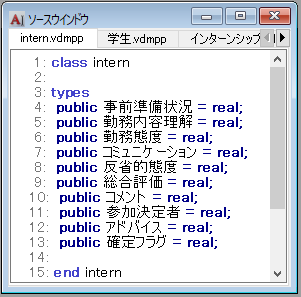
\includegraphics[width=300]{image/speA_vdm1.PNG}
    \caption{仕様書Aから人手によって生成したファイル1}
    \label{fig:speA_vdm1}
    \end{center}
\end{figure}

\begin{figure}[tp]
    \begin{center}
    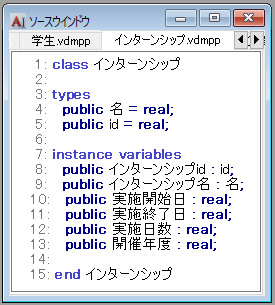
\includegraphics[width=300]{image/speA_vdm2.PNG}
    \caption{仕様書Aから人手によって生成したファイル2}
    \label{fig:speA_vdm2}
    \end{center}
\end{figure}

\begin{figure}[tp]
    \begin{center}
    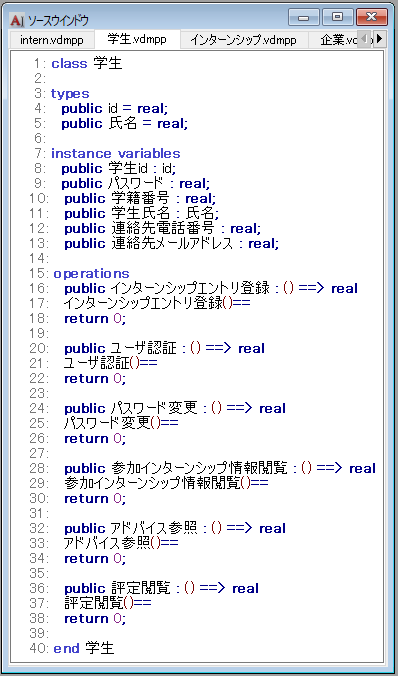
\includegraphics[width=300]{image/speA_vdm3.PNG}
    \caption{仕様書Aから人手によって生成したファイル3}
    \label{fig:speA_vdm3}
    \end{center}
\end{figure}

\begin{figure}[tp]
    \begin{center}
    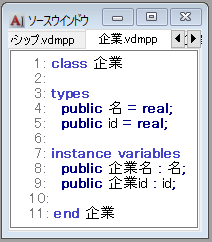
\includegraphics[width=300]{image/speA_vdm4.PNG}
    \caption{仕様書Aから人手によって生成したファイル4}
    \label{fig:speA_vdm4}
    \end{center}
\end{figure}

\begin{figure}[tp]
    \begin{center}
    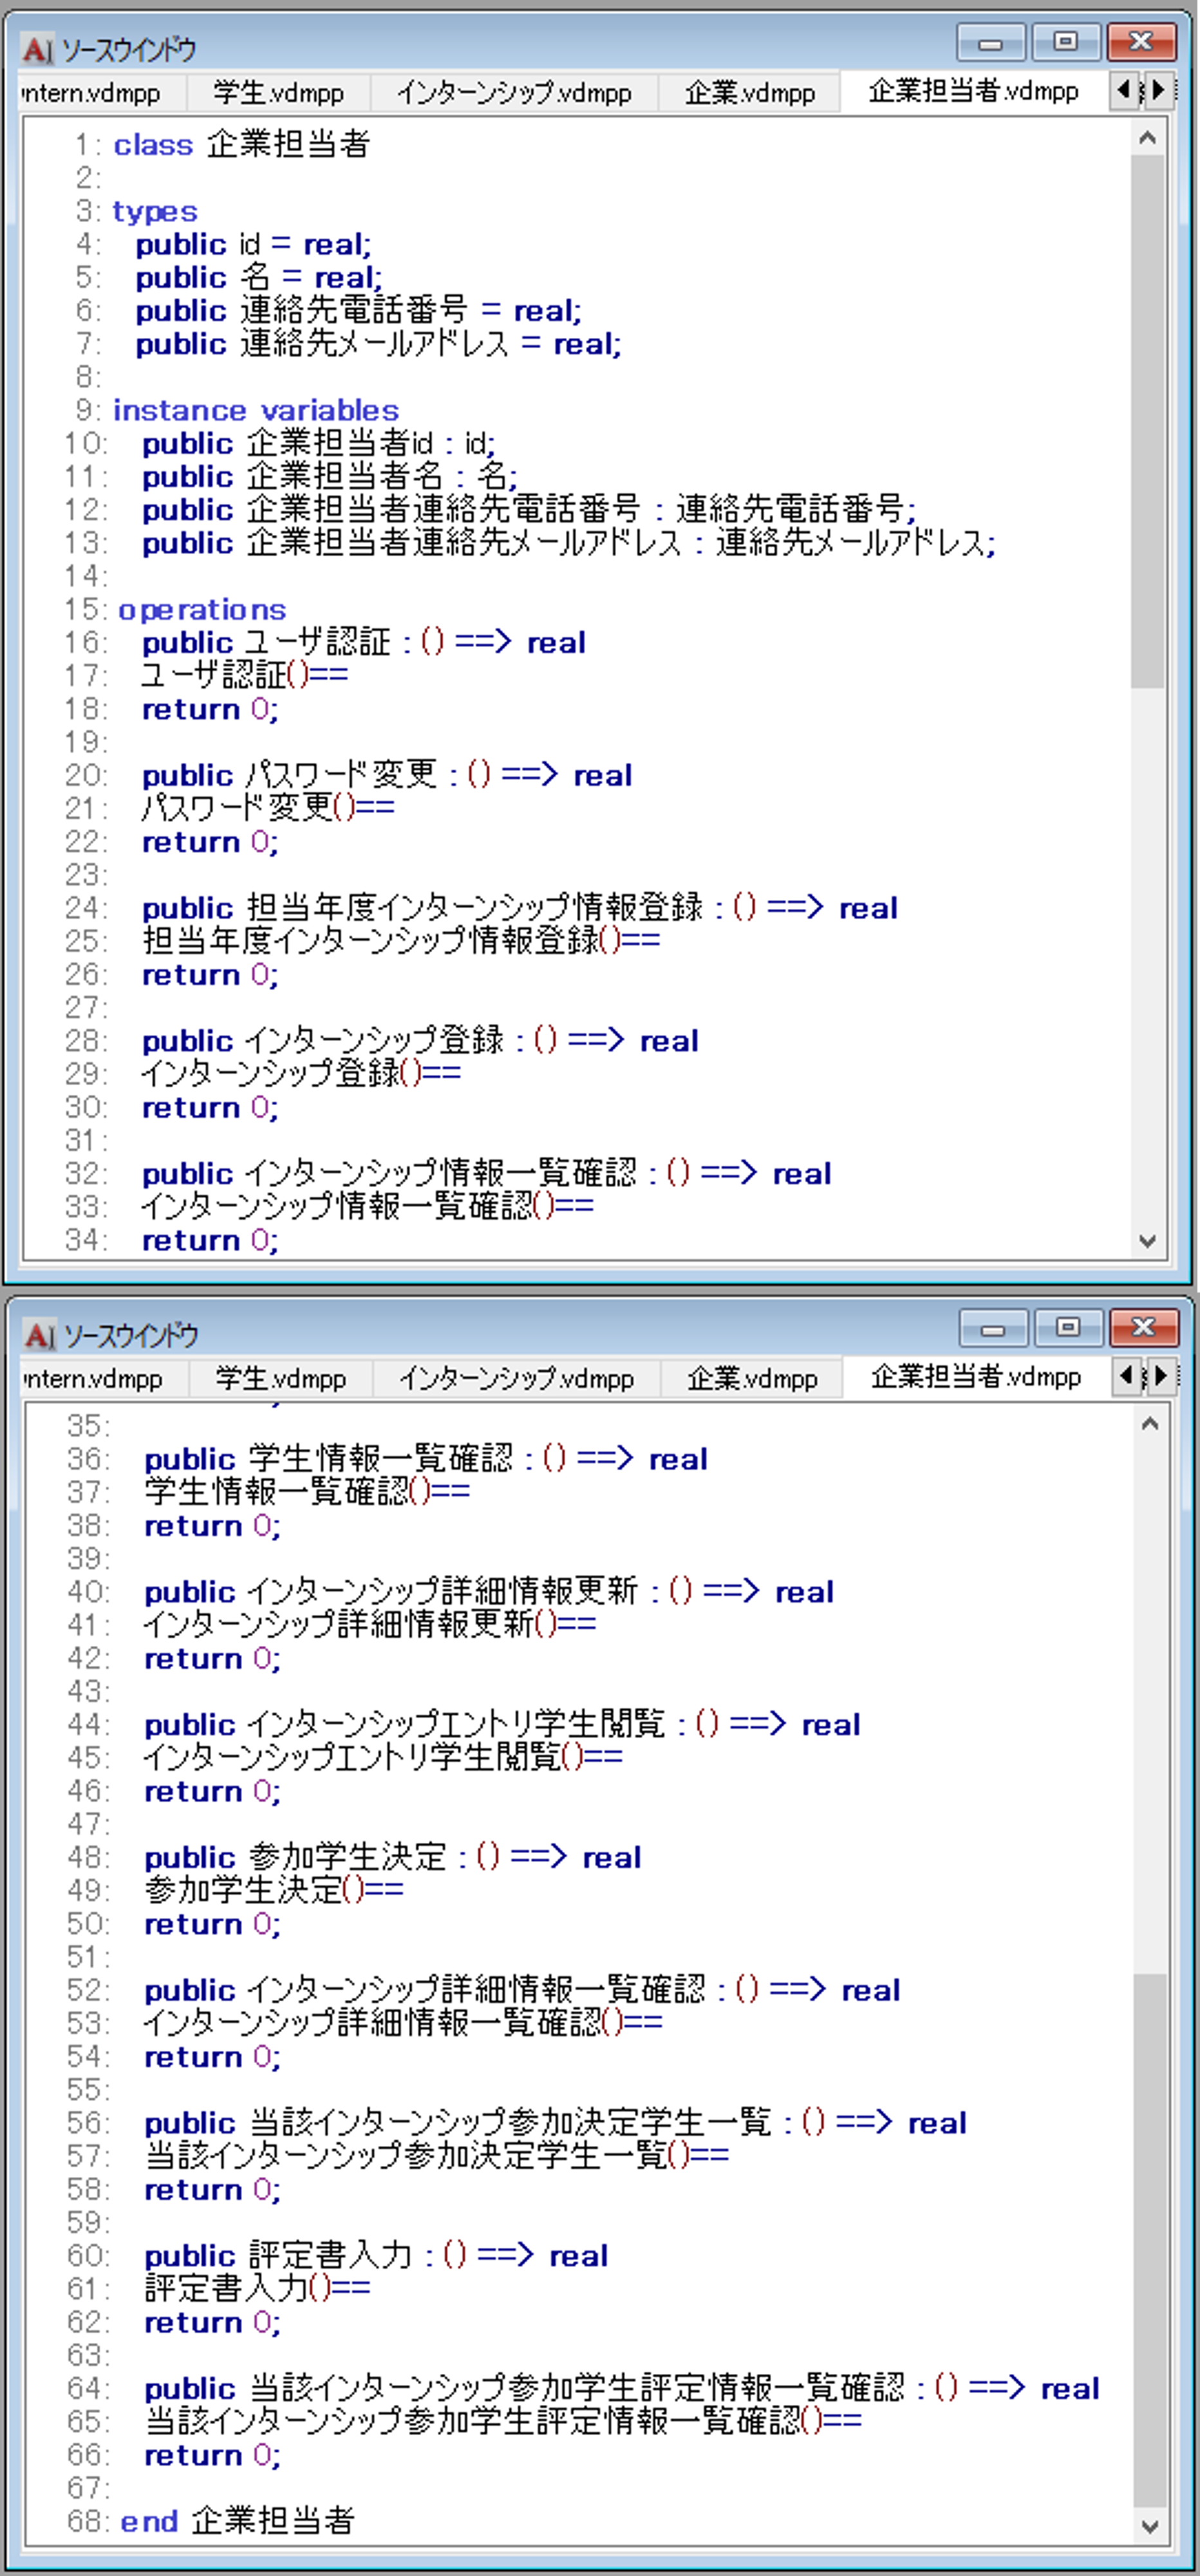
\includegraphics[width=300]{image/speA_vdm5.PNG}
    \caption{仕様書Aから人手によって生成したファイル5}
    \label{fig:speA_vdm5}
    \end{center}
\end{figure}

\begin{figure}[tp]
    \begin{center}
    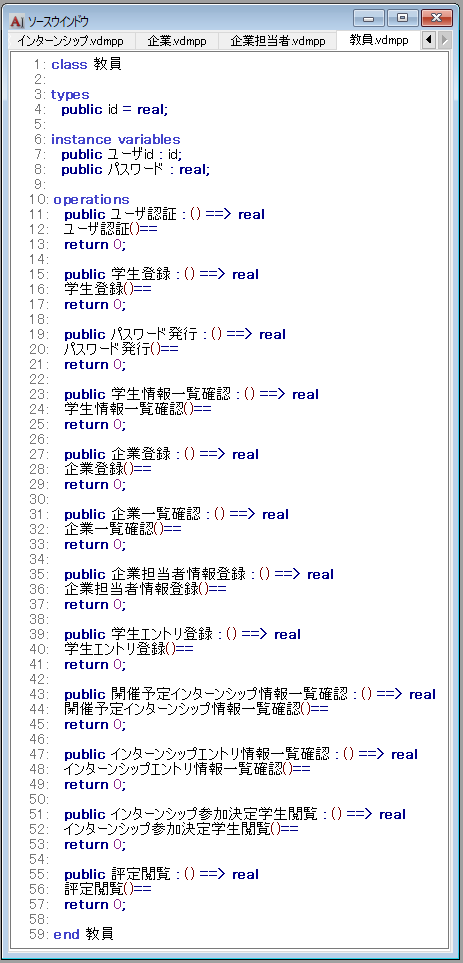
\includegraphics[width=300]{image/speA_vdm6.PNG}
    \caption{仕様書Aから人手によって生成したファイル6}
    \label{fig:speA_vdm6}
    \end{center}
\end{figure}

\begin{figure}[tp]
    \begin{center}
    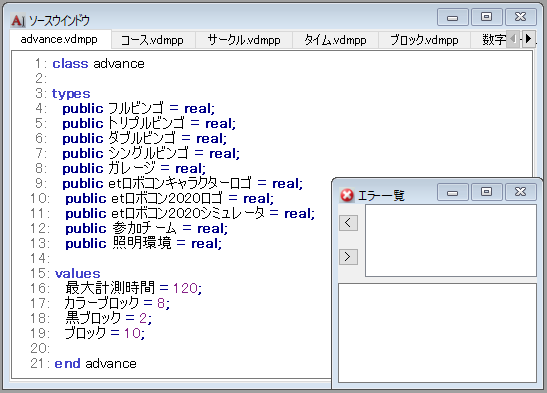
\includegraphics[width=300]{image/speB_vdm1.PNG}
    \caption{仕様書Bから人手によって生成したファイル1}
    \label{fig:speB_vdm1}
    \end{center}
\end{figure}

\begin{figure}[tp]
    \begin{center}
    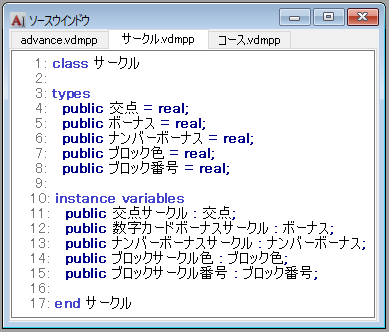
\includegraphics[width=300]{image/speB_vdm2.PNG}
    \caption{仕様書Bから人手によって生成したファイル2}
    \label{fig:speB_vdm2}
    \end{center}
\end{figure}

\begin{figure}[tp]
    \begin{center}
    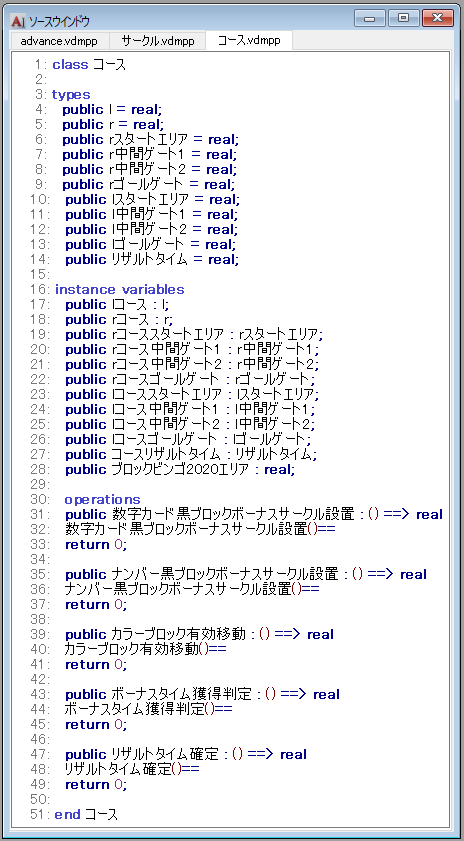
\includegraphics[width=300]{image/speB_vdm3.PNG}
    \caption{仕様書Bから人手によって生成したファイル3}
    \label{fig:speB_vdm3}
    \end{center}
\end{figure}

\begin{figure}[tp]
    \begin{center}
    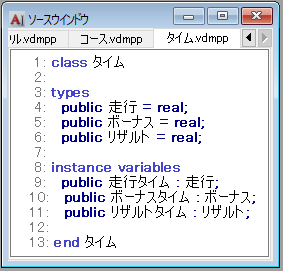
\includegraphics[width=300]{image/speB_vdm4.PNG}
    \caption{仕様書Bから人手によって生成したファイル4}
    \label{fig:speB_vdm4}
    \end{center}
\end{figure}

\begin{figure}[tp]
    \begin{center}
    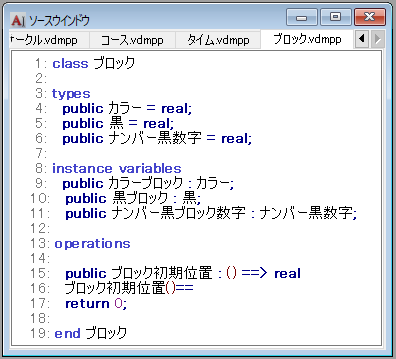
\includegraphics[width=300]{image/speB_vdm5.PNG}
    \caption{仕様書Bから人手によって生成したファイル5}
    \label{fig:speB_vdm5}
    \end{center}
\end{figure}

\begin{figure}[tp]
    \begin{center}
    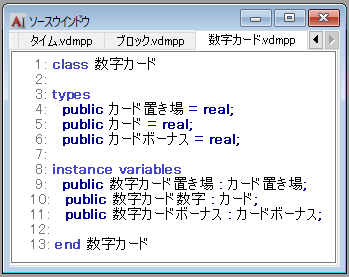
\includegraphics[width=300]{image/speB_vdm6.PNG}
    \caption{仕様書Bから人手によって生成したファイル6}
    \label{fig:speB_vdm6}
    \end{center}
\end{figure}

\begin{figure}[tp]
    \begin{center}
    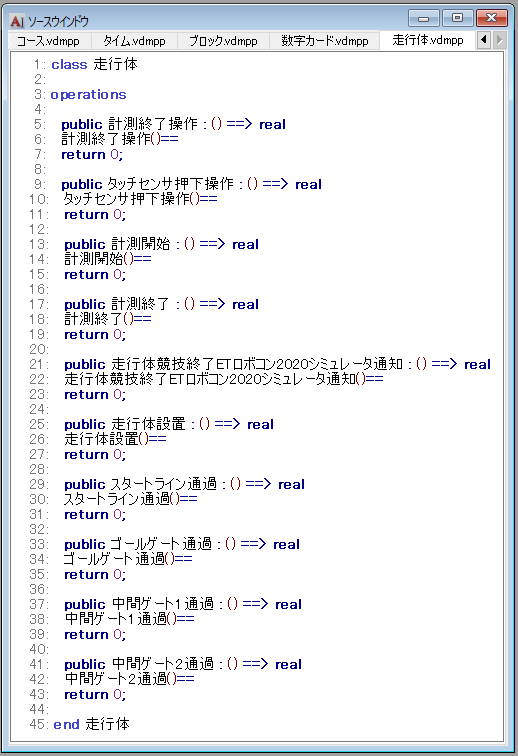
\includegraphics[width=300]{image/speB_vdm7.PNG}
    \caption{仕様書Bから人手によって生成したファイル7}
    \label{fig:speB_vdm7}
    \end{center}
\end{figure}


